\documentclass[10pt,draftclsnofoot,onecolumn]{IEEEtran}
\usepackage{graphicx}
\usepackage{textcomp}
\usepackage{comment}

\graphicspath{ {} }

%TODO need title page from prev documents/ other packages.
% Page layout (geometry)
\setlength\voffset{-1in}
\setlength\hoffset{-1in}
\setlength\topmargin{0.5in}
\setlength\oddsidemargin{.75in}
\setlength\evensidemargin{.75in}
\setlength\textheight{8.278in}
\setlength\textwidth{6.5in}
\setlength\footskip{0.561in}
\setlength\headheight{0.5in}
\setlength\headsep{0.461in}

% Taken from Lena Herrmann at 
% http://lenaherrmann.net/2010/05/20/javascript-syntax-highlighting-in-the-latex-listings-package
\usepackage{listings}
\usepackage{color}
\definecolor{lightgray}{rgb}{.9,.9,.9}
\definecolor{darkgray}{rgb}{.4,.4,.4}
\definecolor{purple}{rgb}{0.65, 0.12, 0.82}

\lstdefinelanguage{JavaScript}{
  keywords={typeof, new, true, false, catch, function, return, null, catch, switch, var, if, in, while, do, else, case, break},
  keywordstyle=\color{blue}\bfseries,
  ndkeywords={class, export, boolean, throw, implements, import, this},
  ndkeywordstyle=\color{darkgray}\bfseries,
  identifierstyle=\color{black},
  sensitive=false,
  comment=[l]{//},
  morecomment=[s]{/*}{*/},
  commentstyle=\color{purple}\ttfamily,
  stringstyle=\color{red}\ttfamily,
  morestring=[b]',
  morestring=[b]"
}

\lstset{
   language=JavaScript,
   backgroundcolor=\color{lightgray},
   extendedchars=true,
   basicstyle=\footnotesize\ttfamily,
   showstringspaces=false,
   showspaces=false,
   numbers=left,
   numberstyle=\footnotesize,
   numbersep=9pt,
   tabsize=2,
   breaklines=true,
   showtabs=false,
   captionpos=b
}


\begin{document}
\pagenumbering{gobble}
\title{Winter Progress Report}
\author{Group 20: Shawn Cross, Paul Kwak, Griffin Gonsalves}
\maketitle
\hspace*{\fill}\IEEEauthorblockA{Capstone - Spring 2017}\hspace*{\fill}
\vspace{2cm}
\begin{abstract}
This document expands upon Group 20's progress with the project as it stands as of the middle of the spring term, and includes a project summary, details of project related problems with changes and solutions, group member evaluations, and a week-by-week breakdown of the progress of the design phase. 
\end{abstract}
\IEEEpeerreviewmaketitle

\newpage
\pagenumbering{arabic}

\section{Project Recap}
%Purposes and Goals
Our project seeks to improve and build upon Vrok.it increasing the usability while simultaneously integrating more functionality using Forge and other APIs. The Forge API collection has several APIs that facilitate development with 3D modeling and creating applications like ours. The end product will be capable of uploading CAD files via local user files or through Data Management’s allowing access to a user’s A360 account, displaying the files as models through the File Viewer, file conversion with the Model Derivative, viewing the site on a mobile device via QR scanner and then viewing the site, specifically models, in VR with Google Cardboard.

Our team is motivated to provide these powerful features and to gain experience developing a larger scale project, in addition to honing programming and teamwork skills. While the foundation is now laid out, we are excited to add more ideas and additional features to our project. For instance, in order to provide support for additional VR devices, we want to ensure the project is useful on a low-cost scenario by utilizing Google's Cardboard headset.

\section{Current Progress}
We have been able to get the Vrok project set up and running on our own web space at https://murmuring-cove-16220.herokuapp.com/. After we were able to get this up and running we began to start implementing our changes to the site. We were able to get the bucket set up that is need for uploading file to the website and make it so that the website will only let user upload certain file types when going through their file on their local machines. We then began to work on the 3-legged authentication required to allow users to get file from there different Autodesk storage services. This is where we began to run into some problems. We found that it was a bit more difficult to do this than we had initially expected. But we were able to find an API that did exactly what we wanted and after talking to one of our mentors Kean of Autodesk we decided that integrating the API into our current website would be the best solution to our problem. Integrating the API was more challenging than we had anticipated but we brought in Adam, the person who created the API to help with the integration. After realizing that we need to update the version of node.js and migrating to the newer versions of the Forge APIs we were able to get Adam's API working with our project for the most part. Once we had the API allowing us to connect to the Autodesk servers we began to get work on getting it to retrieve models from users A360 accounts. This worked well but we ran into difficulty when trying to get the models to show up in the viewer. Once we got this working the next task was to make it so that these models could also be viewed by a participant. This part seemed to give us the most trouble because we had to find a way to pass the information from the main website to the participant. After I finally got this all working the website was mainly complete and we currently working on fixing any bugs we have could find since completion.

\section{Remaining Tasks}
We currently have a few bugs that we are trying to get sorted out. One of the bugs is with the UI and is a problem with two div’s overlapping after a model is loaded into the viewer. The other bugs that we know about might be bugs from the actual forge viewer API and that means we won't be able to fix these bugs ourselves. We can let our client know of the bugs we found so she can inform the Forge API developers at Autodesk. We are also currently working on our pitch and will be recoding that this week to get feedback from our TA before the expo.

\section{Problems and Solutions}
One of the first problems we ran into was getting three-legged authentication working. It turned out that it required a lot more work that we had initially thought it would be. To solve this problem, we decided to use an API that not only allowed us to connect the user to their A360 accounts as wanted it already had a file tree system set up that would let users access their file. First we couldn't gain access to the users A360 account after integrating the API into our project. We found that this was because we were using the wrong version of node.js and once updated we could then connect to A360 as wanted. The next problem we ran into was that we couldn't get the selected model into the viewer even though it was being downloaded properly. It turns out that the viewer being initialized in multiple spots in the program was causing the problem. Our mentor Adam found a solution to this problem and once I implemented it the models could then be loaded into the viewer as wanted. The problem I am working on currently is that once the user picks a model from their A360 account and it is loaded in the viewer they should be able to then have others connect to this same session via the qr code on the website. After the person connects they should be able to see the model that is on the main website. The problem is that the wrong authentication token is being passed to the participant so they can retrieve the model. After discussing the problem with one of our mentors Kean. A solution we found to this problem is to use the socket IO system that was already in place. we created three variables, one boolean to determine if three-legged or two-legged authentication was being used, and then two more that would hold the three-legged token and the time till expiration. We then passed them to the participant and created a callback function to be called by the initializer when they were needed. This solution proved successful and actually proved to work very well. The final problem we ran into was that the viewer wouldn't show the model from a user’s A360 account if they had first chose to look at a model from list. To fix this problem I found that we could just uninitialize the viewer and then reinitialize it every time the user choses a new model.
\section{Code Pieces}

\medskip
\begin{lstlisting}[caption=Exchanging Authorization Code for Token function]
router.get('/api/forge/callback/oauth', function (req, res) {
    var code = req.query.code;
    var tokenSession = new token(req.session);

    // first get a full scope token for internal use (server-side)
    var req = new forgeSDK.AuthClientThreeLegged(config.credentials.client_id, config.credentials.client_secret, config.callbackURL, config.scopeInternal);
    console.log(code);
    req.getToken(code)
        .then(function (internalCredentials) {

            tokenSession.setInternalCredentials(internalCredentials);
            tokenSession.setInternalOAuth(req);

            console.log('Internal token (full scope): ' + internalCredentials.access_token); // debug

            // then refresh and get a limited scope token that we can send to the client
            var req2 = new forgeSDK.AuthClientThreeLegged(config.credentials.client_id, config.credentials.client_secret, config.callbackURL, config.scopePublic);
            req2.refreshToken(internalCredentials)
                .then(function (publicCredentials) {
                    tokenSession.setPublicCredentials(publicCredentials);
                    tokenSession.setPublicOAuth(req2);

                    console.log('Public token (limited scope): ' + publicCredentials.access_token); // debug
                    res.redirect('/');
                })
                .catch(function (error) {
                    res.end(JSON.stringify(error));
                });
        })
        .catch(function (error) {
            res.end(JSON.stringify(error));
        });
});
\end{lstlisting}
\begin{lstlisting}[caption=Package depedencies]
  "dependencies": {
    "socket.io": "*",
    "body-parser": "^1.15.1",
    "cookie-parser": "^1.4.3",
    "ejs": "^2.4.1",
    "express": "^4.13.4",
    "express-session": "^1.13.0",
    "formidable": "^1.0.17",
    "morgan": "^1.7.0",
    "oauth": "^0.9.14",
    "request": "^2.72.0",
    "trim": "0.0.1",
    "forge-apis": "*",
    "jstree": "*"
  },
\end{lstlisting}
\begin{lstlisting}[caption=Login related functions]

function signIn() {
    $.ajax({
        url: '/user/authenticate',
        success: function (rootUrl) {
            console.log("succeeded with sign in" + rootUrl);
            location.href = rootUrl;
        },
        error: function() {
            console.log("Failure at sign in");
        }
    });
}

function logoff() {
    $.ajax({
        url: '/user/logoff',
        success: function (oauthUrl) {
            location.href = oauthUrl;
        }
    });
}

function get3LegToken(callback) {

    if (callback) {
        $.ajax({
            url: '/user/token',
            success: function (data) {
                MyVars.token3Leg = data.token;
                console.log('Returning new 3 legged token (User Authorization): ' + MyVars.token3Leg);
                callback(data.token, data.expires_in);
            },
            error: function() {
                console.log("Err in get3legtoken callback ajax");
            }
        });
    } else {
        console.log('else version of Returning saved 3 legged token (User Authorization): ' + MyVars.token3Leg);

        return MyVars.token3Leg;
    }
}

\end{lstlisting}
\begin{lstlisting}[caption=local file upload restriction]
<input type="file" id="fileElem" style="display:none" accept=".rvt, .iam, .dwfx, .nwc, .dwg, .stp" onchange="onFilesDialogCalled(this.files);" multiple/>
\end{lstlisting}
\begin{lstlisting}[caption=non-local file upload restriction]
function getThreeLeggedScopedOptions(urn){
    var options = {
        'document': 'urn:' + urn,
        'env': 'AutodeskProduction',
        'getAccessToken': get3leggedinfo
    };
    return options;   
}

function get3leggedinfo(callback) {
    console.log("Token: ", _3LegToken);
    console.log("Expires: ", _expires_in);
    callback(_3LegToken, _expires_in);
}
\end{lstlisting}
\begin{lstlisting}[caption=socket.io for passing three legged information]
_socket.emit('lmv-command', { session: _sessionId, name: 'load', value: urn, token: MyVars.token3Leg, expires: MyVars.expires_in, threeLegged: _isThreeLegged });
\end{lstlisting}

\newpage
\begin{figure}[ht]
	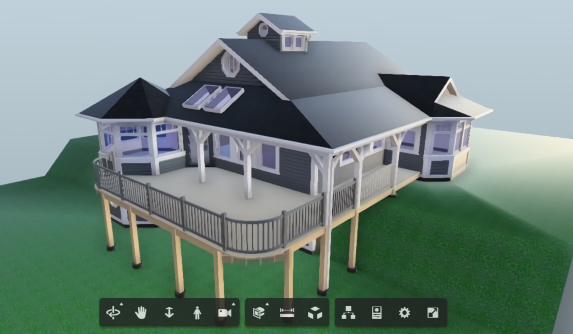
\includegraphics[scale=0.9]{modelviewer.png}
	\caption{Forge's Model Viewer}
\end{figure}
\begin{figure}[ht]
	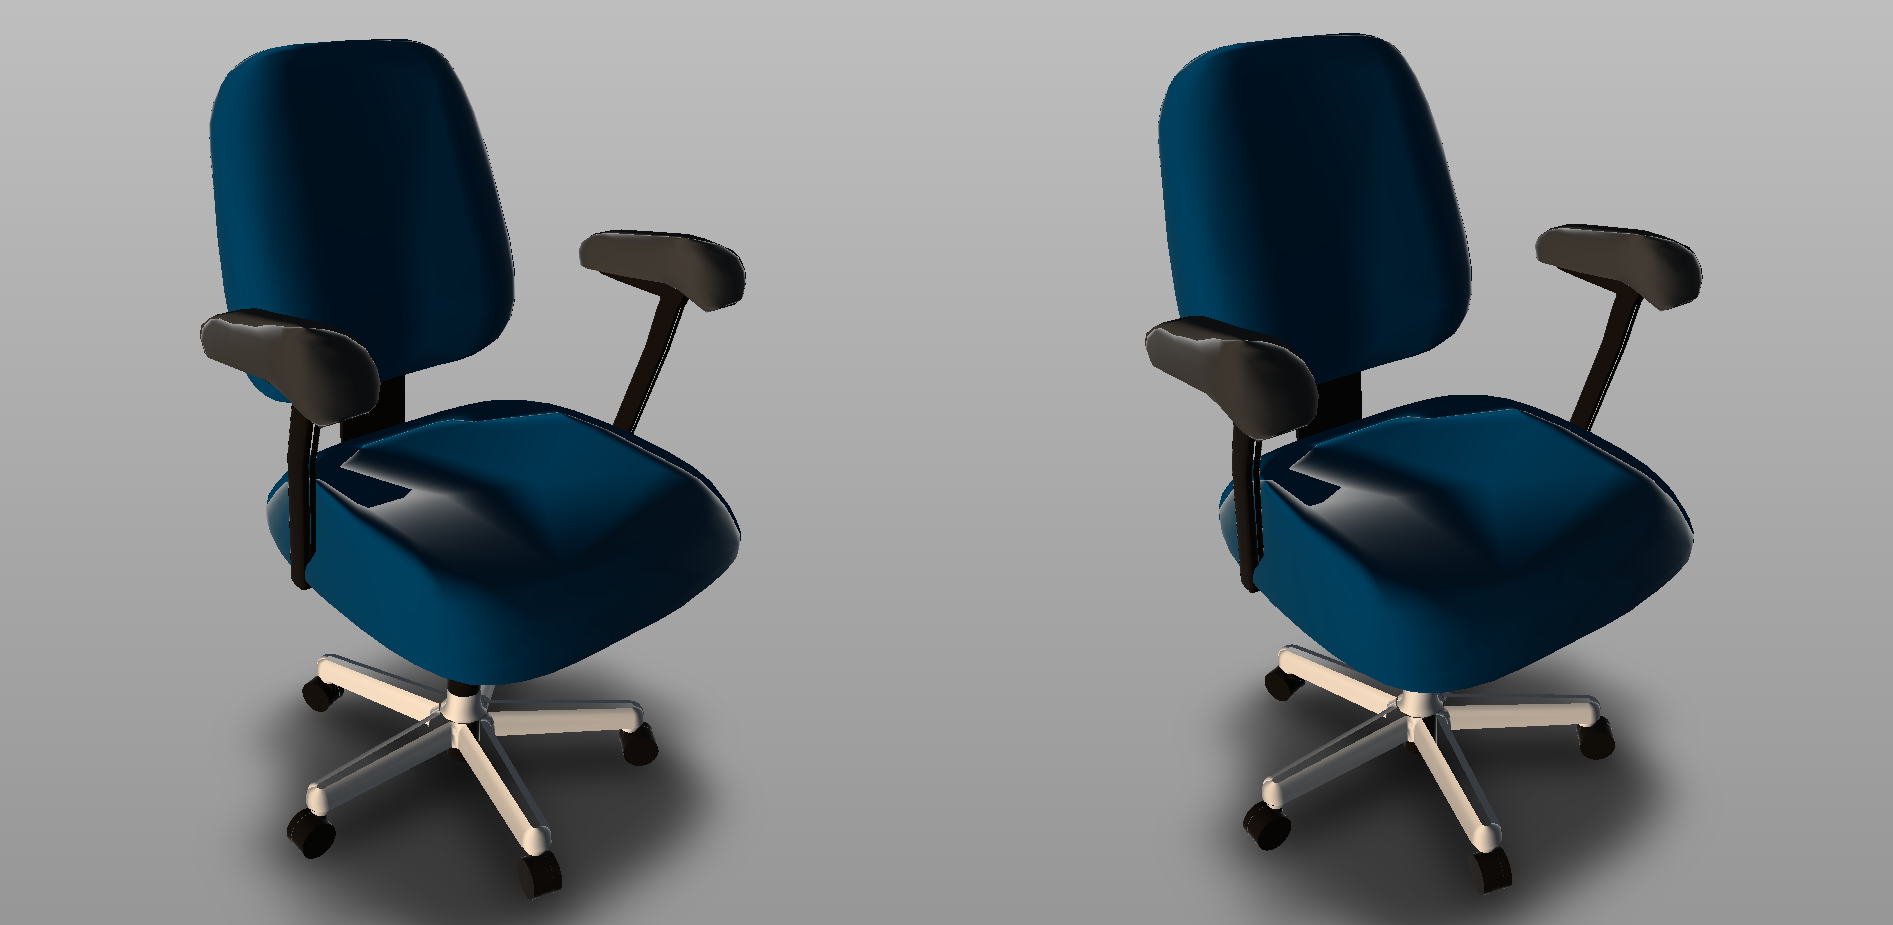
\includegraphics[scale=0.3]{project.png}
	\caption{Stereoscopic View of Model Chair}
\end{figure}

\newpage

\section{Weekly summaries}
\subsection{Week 3}
During this week we were able meet with our client Patti Vrobel and begin to figure out what the we were going to be doing for our project. Patti wanted us to come up with ideas they would make use of the Autodesk Forge APIs. Later that week we had another meeting with Patti and Jim Quanci to figure out if we would be capable of completing the ideas that we had come up with in the time that we had. Jim also gave us a suggestion on what we could do as our project and all of us agreed that the project sounded like something we wanted to do. The biggest issue we had ran into up to this point was trying to get a good idea of what it was exactly that we were going to be doing for our project.   

\subsection{Week 4}
This week we were able to really begin working on our problem statement assignment and start figuring out how exactly we planned on expanding the vrok.it project that we would be starting from. We also had another conference call with Patti and were able to get many of the questions we had about the project cleared up. We were also able to get in contact with the engineer behind the vrok.it project, Kean, and he provided us with more information about what he had intended the project to be. The problem that we were having this week was that we didn't feel like we had an adequate amount of information about what we were actually going to be doing on the project to write a complete problem statement. 

\subsection{Week 5}
During Week 5 we were able to meet up and have a conference call with our client and Kean Walmsley on Monday and Tuesday. During these meetings we were able to complete the project statement and begin preliminary work on the requirements document. It was challenging for us to try to narrow the scope and find more specific goals for the project, and having our group meeting with Patti was very helpful in that regard. At this point we decided to focus more on the user experience end, focusing on usable features, and increasing performance when possible rather than attempting to tackle a challenging optimization. With the fog cleared, we were able to complete the statement document rapidly. In the coming days we were able to use our client meeting to drive our requirements document, and laid out some of the fundamental ideas, such as the viewer and VR content.

\subsection{Week 6}
Week 6 we had hoped to be able to meet with our client to go over some of the details of our project that we were still unsure about, however we were unable to do so. We had also talked with our TA Nels about joining us on our next conference call with the client to help us figure out if what the client was wanting us to do was actually possible in the amount of time that we have. At this point the biggest problem we had was that we were not able to communicate with our client very well because they were in the process of getting ready for a big conference that they host every year. This was challenging for us because we had a lot of questions about the project and the requirements but we were unable to get them answered.

\subsection{Week 7}
During this week we were finally able to get a draft of our requirements document done and get feedback from Nels. His biggest suggestion to us was to be more detailed in the descriptions of our specific requirements. We also had come up ways in which we could use more of the Autodesk APIs, so we also wanted to add those to the final version of the document that we would be turning in as well. We were able to get a hold of Patti this week and set up a conference call with everyone for some time during the next week. We were all looking forward to finally getting to talk to everyone and hopefully get all of the questions at this point answered. The technology review assignment also began during this week. The biggest problems we had during this week were trying to finish the revision of our requirements document and do our individual tech reviews at the same time. Also Paul was very sick this week and was unable to help as much as he normally would. 

\subsection{Week 8}
This week started with the tech reviews being turned in. As a group we all had the same feeling that while the individual reviews we did weren't bad they could have definitely been better if we had a little more time. Although a bit time consuming we did find the tech reviews to be useful in figuring out exactly how we planned on completing each of our individual tasks. We were also set up to have a conference call with Patti and the other people involved with the project to close out the week. Nels was also going to join us for this call to help us determine if some of the performance stuff that Jim had suggested we try to do was something we could actually accomplish. Overall this was a very productive week for our group and we all felt like we were finally starting to get caught back up this week. We did not run into to many problems during this week other than some minor things while trying to do our individual tech reviews. 

\subsection{Week 9}
This week was probably the least productive week of the term for our group. This was the week of thanksgiving so we were all doing some traveling and trying to spend time with our families. We did however try to start the design document that was due the following Friday. This is where we ran into one of the biggest problems we had trying to do this assignment and that was understanding the information in the IEEE document that we were using for this assignment. As a group we were able to get a start on the document but did not get nearly as far on it as we had hoped to over the long weekend. We did manage to have a conference call with everyone to start the and got a lot of the questions that we still had answered. This allowed us to finish the final draft of our requirements document and get the document turned into Nels and Kirsten.  

\subsection{Week 10}
You could definitely tell that this term was coming to an end this week with everyone in our group running out of steam. We all had a ton of assignments and projects due this week and at the beginning of the next week and were all getting very little sleep trying to get it all done. In this class the design document was due on Friday by noon and we all really wanted to have it done by that deadline. We were still having problems trying to figure out how to use the IEEE 1016 doc at the beginning  of this week but we were able to talk to both Kirsten and Nels and really get a good idea of how to actually use the information in the 1016 to create a good design document. After that we were really able to get going on the document and we all spent a lot of time during this week adding to and revising the document and in the end we thought that the document had turned out to be really well done with a lot of good information for both us and our client. 

\subsection{Winter Week 1}
Shawn Cross - This week we didn't get much accomplished but we were able to start setting up the website in our own web space. We had planned on using github.io to host the website but we quickly ran into problems since the website needed a server to run properly and github.io doesn't not offer the ability to run one. We contacted Kean about where a good place to host the site and he told us that we should run it on heroku since the have server capability and it is free. I think overall I would have liked to accomplish more this week but I felt like we were still in a good place as far as our timeline was going.

Paul Kwak- With new schedules our group wasn't able to meet. We could only exchange schedules and try to set impromptu meetings. We also scambled to get client meetings with Patti setup again, depsite the new school schedules. Our first main order of business was to begin getting Kean's website up and running. We weren't really sure how to do this but knew it was the biggest start we could have going into the term. Since once we had it setup we could start making the changes we needed to.

Griffin Gonsalves - Following our initial plan for updating the design, I began with opening up the project files to understand more of the backend, and how each project file was related to each other. I have designed and implemented a few different web sites before, but I hadn't worked on a server-based node.js project like this.  I began implementing the site through GitHub hosting, and the initial page began to load after my first week of work on the site. As it turned out, I was not necessarily prepared for all of the learning of the tools that were suddenly thrust upon me. However, we soon discovered that GitHub hosting was inadequate for our project as the node resources require a server interface. I was very unfamiliar with the node tools, and Heroku page setup as they are both robust and powerful applications, but learned enough to assist move the project off of the GitHub Pages site. I was a bit bummed that the initial plan didn't work out as we had hoped, but I think the result is perfectly fine-the site has not had any major hosting issues since the transition.

\subsection{Winter Week 2}
Shawn Cross- This week I found that getting the site up and running completely was proving to be more difficult than I had initially thought that it was going to be. I had gotten a heroku account set up and got it installed on my computer along node.js, since that is what we would be using for the backend. After that I was get the website setup on our heroku domain by initializing heroku in our git repo and then pushing all the website file to heroku. Once the files were pushed the site began working for the most part but I had forgotten to add our credentials from my forge app so the site wouldn't load completely. Putting the credentials in was the last thing I needed to get the website to load completely. Overall I felt like even with the problems I ran into getting the website set up I did learn a lot and got quite a bit done this week. 

Paul Kwak - We initially began by trying to host Kean's files via gitpages. This did not work what so ever. When asking Kean, he told us he used Heroku to host Vrok.it and all the code was already setup to work with Vrok.it. We had several issues even while trying work with Heroku. One issue was his code utilized standard HTTP urls. This gave us many security errors, so it was a simple change to HTTPS. The second issue we had was getting the Heroku to setup correctly mostly due to his credentials not being changed to the ones we should have been using. Once these issues were smoothed, we had to figure out how to update the files we changed to Heroku. We basically set it up so our git repo can be directly uploaded to Heroku. This particular week we did not meet with Patti, but did setup a meet on the next week to talk about progress and also get some smaller questions answered.

Griffin Gonsalves - During week 2 of our development phase, we made a transition to Heroku for our hosting service. This change delayed us slightly, but overall is for the better since we now have a server to push our project files to. During this week we reached out to our project sponsor at Autodesk, Patti Vrobel, to assist us in this setup. We also began planning our transition to our next phase of development on our schedule. Each of us spent time learning Git essentials for our machines, and set up so we could each push updates to the server. I have begun doing more investigation with project files and how we will navigate with multiple viewers active at once. Once we are able to test out key functions of the site I plan on beginning to update the site layout next week.
\subsection{Winter Week 3}
Shawn Cross - This week I found that I needed to create a bucket to put the files into so that they could be loaded by the viewer. I had asked Kean how to do this and he suggested that I use curl. I began trying to figure this out but found that I was unable to get the curl commands to work the way I thought they were supposed to. I did some searching and found a website that would actually create the bucket for you by essentially running the curl commands for you. This was very convenient and made the process much simpler. After I had the bucket created I placed a couple model files into the bucket and added them to the list on the site to test that it was working properly and it did they loaded up in the viewer as hoped. I then checked that the upload feature was working properly with our new bucket and was pleased when the first model I tried to upload worked exactly as it was supposed to. We also had our first conference call with Patti and Kean this week and got many of the questions that we had come up with since the beginning of the term answered. I felt pretty accomplished this week was excited that we were finally to the point where we could start implementing the changes we had planned for the site.

Paul Kwak - We met with Patti and also Kean, the creator of Vrok.it. However, for the meeting the only person who had any questions was Shawn, as he was the one working with getting the buckets and file formatting working. Who didn't end up being able to make it. Overall the meeting was somewhat unfruitful. In the end Shawn was able to get the file upload and site up and running perfectly. After this it was my job to get the authentication running. In the actual Autodesk tutorial it gave an href with a link that would redirect a user to receive a Authorization code which could then be sent to receive a token. I was able to get this work just fine. The rest of the tutorial was extrememly unhelpful, there were only descriptions of what to do next and no code samples. I had very little Javascript experience so I had to search online in order to accomplish what I needed. So the Authorization code parameter was given through the URL, but Kean's QR code would actually set the URL to a session which would wipe out the code almost instantly. I had to create a script that would parse through the URL and once it matched on a "=" symbol would take split the URL. Then it would take the latter half and keep that saved. Unforunately the session also had an "=" symbol but that was easily fixable through a if statement. While I was able to retrieve the code from the URL the next section of the tutorial used php, and I had to begin learning up on ajax.

Griffin Gonsalves - Another week down, and things have begun to pick up more speed. We were able to meet again with our client and Kean Walmsley from Autodesk via conference call, and got heaps of useful information on the site and some guidance for our development. After setting up our upload pipeline for Heroku, I started planning out what some of the layout changes could be and what I wanted the site to end up looking like. I spent some time brushing up on node.js, and some of its useful features. At the beginning of next week I hope to begin pushing some changes to the site so that the layout will be adjusted and some other site features can be added later down the line. Additionally, we hope to have an updated development schedule early in the week.
\subsection{Winter Week 4}
Shawn Cross - To start this week, I was able to get local file type restriction working. This turned out to be a lot easier than I had initially thought that was going to be since it turned out all I had to was add an attribute to the file tag that specified the types of files that we were going to allow. After I had this working I began working with Paul to get the 3-legged authentication since my next task was to get non-local file uploading to work but could not do until we had the 3-legged working. Paul had initially planned on writing this part from scratch but we quickly realized that doing it that way would take a ton of work and a ton of code to do. After some searching we discovered an API that not only did the 3-legged authentication it also had a file tree system for navigating through peoples' files from their outside storage. During our conference call with Kean we determined that using the API would be the best option for us since it did exactly what we wanted. We began trying to integrate the API but began running into problems since neither of us had much experience with javascript or web development in general. I would say that overall this week was ok it was kind of frustrating that we weren't able to get as much of the integration working as we had really hoped. 

Paul Kwak - Trying to follow up on the work I had done in the previous week was reading up on XMLHTTPrequests as well as ajax. I had a decent amount of midterms that week so I wasn't able to get much work done. It was during this week we found a website with accompanied git repository that had all the functionality we were looking for. We began dissecting his code to understand what was going on. It was here I realized that  in a way, I had been doing the authentication wrong. The code had the Data Management, Model Derivative APi and Data Authentication API in a server side. WIth my lack of experience in web I didn't even realize that the server side was keeping all important data hidden from the client side. Which I was had been mostly debugging through the inspect function in chrome. I also began using the Heroku server logs to begin an additional layer of debugging. The server file utilizes express.js and has matching on ajax requests. I began breaking down the API.

Griffin Gonsalves - Overall, this week was not quite as smooth as we had hoped, but still progress is being made nonetheless. Spending more time with the project, I discovered that the main landing page is actually a compilation of pages being loaded at once, making the adjustment of the layout more complex than I had originally thought. I suspect this has to do with node running a live session and pages loading in asynchronously. I have the removal and updating of several pages for the project site near-ready, however, I had to wait until Paul and Shawn were completing their portions of the project. I hope to push these updates next week and start working with the team and Autodesk on A360 integration and possibly on the movement within the Autodesk Viewer. Hopefully this week we'll be able to do some testing with our Google Cardboard as well with the new models, and various model types early this week so we can develop a more optimal setup for the Viewer on our page. Overall, I think the website will look great once the authentication changes have been completed.
\subsection{Winter Week 5}
Shawn Cross - During this week we were still working on the API integration and it was still proving to be more dificult than we had anticipated. During our conference call with Kean we found out that he knew the person that created the API that we were trying to integrate and offered to reach out to him and see if he would be willing to help us with the integration. This was really exciting since we had been having so much trouble figuring out how all of the different parts were working together. Kean had suggested that while waiting to see if Adam would be willing to help us we should keep trying to get the integration working. Paul was able to make progress on this but got to a point where a code that was being returned was not being used by the javascript like it was expected to and neither of us could figure out why that was happening. This week was pretty disappointing since we were not able to get as much done as any of us had hoped however we were excited that we may have the help we needed to figure out what the problems were with the integration. 

Paul Kwak - During this week I began putting together Kean's code and the API we found. This took place in two steps, in the first step I had to essentially put the two server files and combine them into 1 file. Second I had to combine the package.json file between the two as that file provides Heroku the dependencies that the server requires in order to run. After testing and time I was able to get the two working. I say that in one sentence but there were tons of problems. One of the problems that existed after getting the site to work was that the login button did not work. I deployed the original website via a separate Heroku app project that works fine. However, ours when using the websites HTML does not redirect the user properly to Autodesk login page. When hardcoding the URL it does redirect, but does not return a token properly as the original website does. I am still trying to get this to work properly and think there is still some conflict between the two server files.

Griffin Gonsalves - This week I was a bit bogged down in other classwork, but I was still able to contribute to our project and help the team. I'm very glad that Paul and Shawn were able to make significant progress on the authentication for the site, and now we shouldn't have any other significant setbacks moving forward. During this week, I developed a new prototype for the website layout, now that we have updated our design with our current technology and have tested our authentication properly. It is exciting to see the project come together so suddenly, and that we are all getting more ideas while we are developing. I hope in the next week after we complete our necessary progress report documentation that we will be able to get creative and put some awesome work into the project for the rest of development. In order to do this, we plan on meeting again with our friends at Autodesk via phone call or Skype during week 6 and 7 in order to address any pressing questions we may have with APIs or our project in general.

\subsection{Winter Week 6}
Shawn Cross - This week Kean was able to get of ahold of Adam, the person who created the API we will be integrating into our project that will handle the non-local file upload. We spent a lot of this week getting the midterm progress report done so we didn't end up getting as much stuff done on the project during this week. 

\subsection{Winter Week 7}
Shawn Cross - We were able to get the authentication working during this week with the help of Adam. We found that we were using the wrong version of node.js and once updated the authentication began to work. The file tree system still wasn't working properly though so my task this week was to try to figure this out. I spent the week working with Adam trying to figure out what was causing the problem. We were able to figure out that the versions of the Forge APIs that we were using were not the most recent versions and that we needed to migrate them to the newer versions.

\subsection{Winter Week 8}
Shawn Cross - Adam helped me to get the APIs migrated to the newer versions and we were able to get the file tree system working once this was done. This was exciting for us since we had spent a long time trying to get this API integrated. Now that users could get connected to their A360 accounts and navigate through their files we need to get it so their models would show up in the viewer. I spent the rest of this week trying to figure out why this wasn't working. After working with Adam, we discovered that it had to do with the initialization of the viewer. He came up with a work around that I then implemented and we were successful at getting the models to load into the viewer.

\subsection{Winter Week 9}
Shawn Cross - This week I spent working with Kean trying to figure out the latest problem that I had run into. After a lot of debugging I found that the wrong token was being passed to the participant and that we need to find a way to pass a different token to the participant. After emailing back and forth with Kean we came up with a solution that might solve this problem and I began working on getting this implemented. We also got the second draft of our poster done during this week.

\subsection{Winter Week 10}
Shawn Cross - During this week we spent most of our time working on the final progress report. Everyone in the group was also working on projects for other classes and preparing for our finals. Due to working on stuff for other classes we were not able to do as much work on the capstone project as we had all hoped. I was able to further figure out how to get the token to the participant this week. I will spend the break trying to get this implemented into the project so that we can begin to prepare for the expo.

\end{document}
